\documentclass[table]{beamer}
%[]中可以使用draft、handout、screen、transparency、trancompress、compress等参数

%指定beamer的模式与主题
\mode<presentation>
{
  \usetheme{Madrid}
%\usetheme{Boadilla}
%\usecolortheme{default}
%\usecolortheme{orchid}
%\usecolortheme{whale}
%\usefonttheme{professionalfonts}
}

%\usetheme{Madrid}
%这里还可以选择别的主题:Bergen, Boadilla, Madrid, AnnArbor, CambridgeUS, Pittsburgh, Rochester, Warsaw, ...
%有导航栏的Antibes, JuanLesPins, Montpellier, ...
%有内容的Berkeley, PaloAlto, Goettingen, Marburg, Hannover, ...
%有最小导航栏的Berlin, Ilmenau, Dresden, Darmstadt, Frankfurt, Singapore, Szeged, ...
%有章和节表单的Copenhagen, Luebeck, Malmoe, Warsaw, ...

%\usecolortheme{default}
%设置内部颜色主题(这些主题一般改变block里的颜色);这个主题一般选择动物来命名
%这里还可以选择别的颜色主题,如默认的和有特别目的的颜色主题default,structure,sidebartab,全颜色主题albatross,beetle,crane,dove,fly,seagull,wolverine,beaver

%\usecolortheme{orchid}
%设置外部颜色主题(这些主题一般改变title里的颜色);这个主题一般选择植物来命名
%这里还可以选择别的颜色主题,如默认的和有特别目的的颜色主题lily,orchid,rose

%\usecolortheme{whale}
%设置字体主题;这个主题一般选择海洋动物来命名
%这里还可以选择别的颜色主题,如默认的和有特别目的的颜色主题whale,seahorse,dolphin

%\usefonttheme{professionalfonts}
%类似的还可以定义structurebold,structuresmallcapsserif,professionalfonts

% 控制 beamer 的风格,可以根据自己的爱好修改
%\usepackage{beamerthemesplit} %使用 split 风格
%\usepackage{beamerthemeshadow} %使用 shadow 风格
%\usepackage[width=2cm,dark,tab]{beamerthemesidebar}

%插入音标
%\usepackage{tipa}
%\AtBeginDocument{
  %\renewcommand\textipa{\fontencoding{T3}\selectfont}
%}
%\AtBeginDocument{
  %\renewcommand\textipa[2][r]{{\fontfamily{cm#1}\tipaencoding #2}}
%}
%\renewenvironment{IPA}[1][r]
 %{\fontfamily{cm#1}\tipaencoding}
 %{}

% 设定英文字体
%\usepackage{fontspec}
% Fix bugs for fontspec in TeXLive2015
\ifdefined\suppressfontnotfounderror
  \expandafter\let\csname xetex_suppressfontnotfounderror:D\endcsname
    \suppressfontnotfounderror
\else
  \expandafter\let\csname xetex_suppressfontnotfounderror:D\endcsname
    \luatexsuppressfontnotfounderror
\fi
\usepackage[no-math]{fontspec}
\setmainfont{Times New Roman}
\setsansfont{Arial}
\setmonofont{Courier New}

% 设定中文字体
\usepackage[BoldFont,SlantFont,CJKchecksingle,CJKnumber]{xeCJK}
%\setCJKmainfont[BoldFont={Adobe Heiti Std},ItalicFont={Adobe Kaiti Std}]{Adobe Song Std}
\setCJKmainfont[BoldFont={Adobe Heiti Std},ItalicFont={Adobe Kaiti Std}]{WenQuanYi Micro Hei}
\setCJKsansfont{Adobe Heiti Std}
\setCJKmonofont{Adobe Fangsong Std}
\punctstyle{hangmobanjiao}

\defaultfontfeatures{Mapping=tex-text}
\usepackage{xunicode}
\usepackage{xltxtra}

\XeTeXlinebreaklocale "zh"
\XeTeXlinebreakskip = 0pt plus 1pt minus 0.1pt

\usepackage{setspace}
\usepackage{colortbl,xcolor}
\usepackage{hyperref}
%\hypersetup{xetex,bookmarksnumbered=true,bookmarksopen=true,pdfborder=1,breaklinks,colorlinks,linkcolor=blue,filecolor=black,urlcolor=cyan,citecolor=green}
\hypersetup{xetex,bookmarksnumbered=true,bookmarksopen=true,pdfborder=1,breaklinks,colorlinks,linkcolor=cyan,filecolor=black,urlcolor=blue,citecolor=green}

% 插入图片
\usepackage{graphicx}
\graphicspath{{figures/}}
% 图文混排
%\usepackage{picins}
\usepackage{floatflt}

% 可能用到的包
\usepackage{amsmath,amssymb}
%插入多媒体
%\usepackage{media9}
%\usepackage{movie15}
\usepackage{multimedia}
\usepackage{multicol}
\usepackage{multirow}

% 定义一些自选的模板,包括背景、图标、导航条和页脚等,修改要慎重
% 设置背景渐变由10%的红变成10%的结构颜色
%\beamertemplateshadingbackground{red!10}{structure!10}
%\beamertemplatesolidbackgroundcolor{white!90!blue}
% 使所有隐藏的文本完全透明、动态,而且动态的范围很小
\beamertemplatetransparentcovereddynamic
% 使itemize环境中变成小球,这是一种视觉效果
\beamertemplateballitem
% 为所有已编号的部分设置一个章节目录,并且编号显示成小球
\beamertemplatenumberedballsectiontoc
% 将每一页的要素的要素名设成加粗字体
\beamertemplateboldpartpage

% item逐步显示时,使已经出现的item、正在显示的item、将要出现的item呈现不同颜色
\def\hilite<#1>{
 \temporal<#1>{\color{gray}}{\color{blue}}
    {\color{blue!25}}
}

\renewcommand{\today}{\number\year 年 \number\month 月 \number\day 日}

%五角星
\usepackage{MnSymbol}

%去除图表标题中的figure等
\usepackage{caption}
\captionsetup{labelformat=empty,labelsep=none}

\usepackage{tabu}
\usepackage{multirow}
%表格自动换行
\usepackage{tabularx} 

% 千分号
%\usepackage{textcomp}

%罗马数字
\makeatletter
\newcommand{\rmnum}[1]{\romannumeral #1}
\newcommand{\Rmnum}[1]{\expandafter\@slowromancap\romannumeral #1@}
\makeatother

%分栏
\usepackage{multicol}

%\usepackage{enumitem}
%\usepackage{enumerate}

%键盘
\usepackage{keystroke}

%插入源代码
\usepackage{listings}
\lstset{
  language=perl,                  % 程序语言名称:TeX, Perl, R, sh, bash, Awk
  basicstyle=\normalsize\tt,      %\tt指monospace字体族,程序源代码使用此族字体表示更加美观
  numbers=left,                   % 行号位置(左侧)
  numberstyle=\small,             % 行号字体的字号
  stepnumber=1,                   % 行号的显示步长
  numbersep=5pt,                  % 行号与代码间距
  backgroundcolor=\color{white},  % 背景色;需要 \usepackage{color}
  showspaces=false,               % 不显示空格
  showstringspaces=false,         % 不显示代码字符串中的空格标记
  showtabs=false,                 % 不显示 TAB
  tabsize=4, 
  frame=shadowbox,                % 把代码用带有阴影的框圈起来
  captionpos=b,                   % 标题位置
  breaklines=true,                % 对过长的代码自动断行
  breakatwhitespace=false,        % 断行只在空格处
  extendedchars=false,            % 解决代码跨页时,章节标题,页眉等汉字不显示的问题
  %escapeinside={\%*}{*},         % 跳脱字符,添加注释,暂时离开 listings 
  %escapeinside=``,
  commentstyle=\color{red!50!green!50!blue!50}\tt,  %浅灰色的注释
  rulesepcolor=\color{red!20!green!20!blue!20},     %代码块边框为淡青色
  keywordstyle=\color{blue!70}\bfseries\tt,         %代码关键字的颜色为蓝色,粗体
  identifierstyle=\tt,
  stringstyle=\tt,                % 代码字符串的特殊格式
  keepspaces=true,
  breakindent=1em,
  %breakindent=22pt,
  %breakindent=4em,
  breakautoindent=true,
  flexiblecolumns=true,
  aboveskip=1em,                  %代码块边框
  xleftmargin=2em,
  xrightmargin=2em
}

%\setbeamercolor{alerted text}{fg=magenta}
\setbeamercolor{bgcolor}{fg=yellow,bg=cyan}
%\setbeamercolor{itemize/enumerate body}{fg=green}

\begin{document}

%\includeonlyframes{current}

\logo{
\includegraphics[height=0.08\textwidth]{tijmu.png}}

% 在每个Section前都会加入的Frame
\AtBeginSection[]
{
  \begin{frame}<beamer>
    %\frametitle{Outline}
    \frametitle{教学提纲}
    \setcounter{tocdepth}{3}
    \begin{multicols}{2}
      \tableofcontents[currentsection,currentsubsection]
      %\tableofcontents[currentsection]
    \end{multicols}
  \end{frame}
}
% 在每个Subsection前都会加入的Frame
\AtBeginSubsection[]
{
  \begin{frame}<beamer>
%%\begin{frame}<handout:0>
%% handout:0 表示只在手稿中出现
    \frametitle{教学提纲}
    \setcounter{tocdepth}{3}
    \begin{multicols}{2}
    \tableofcontents[currentsection,currentsubsection]
    \end{multicols}
%% 显示在目录中加亮的当前章节
  \end{frame}
}

% 为当前幻灯片设置背景
%{
%\usebackgroundtemplate{
%\vbox to \paperheight{\vfil\hbox to
%\paperwidth{\hfil
\includegraphics[width=2in]{tijmu_charcoal.png}\hfil}\vfil}
%}
\begin{frame}[plain]
  \begin{center}
    {\Huge 分子生物计算\\}
    {\huge \textit{(Perl语言编程)}\\}
    \vspace{1cm}
    {\LARGE 天津医科大学\\}
    %\vspace{0.2cm}
    {\LARGE 生物医学工程与技术学院\\}
    \vspace{1cm}
    {\large 2016-2017学年上学期(秋)\\ 2014级生信班}
  \end{center}
\end{frame}
%}



\title[编程的艺术]{第三章\quad 编程的艺术}
\author[Yixf]{伊现富(Yi Xianfu)}
\institute[TIJMU]{天津医科大学(TIJMU)\\ 生物医学工程与技术学院}
\date{2015年9月}

\begin{frame}
  \titlepage
\end{frame}

\begin{frame}[plain,label=current]
  \frametitle{教学提纲}
  \setcounter{tocdepth}{3}
  \begin{multicols}{2}
    \tableofcontents
  \end{multicols}
\end{frame}


\section{引言}
\begin{frame}
  \frametitle{编程艺术 | 引言}
  \begin{figure}
    \centering
    
\includegraphics[width=0.41\textwidth]{c3.programming.c.01.jpg}
    \quad
    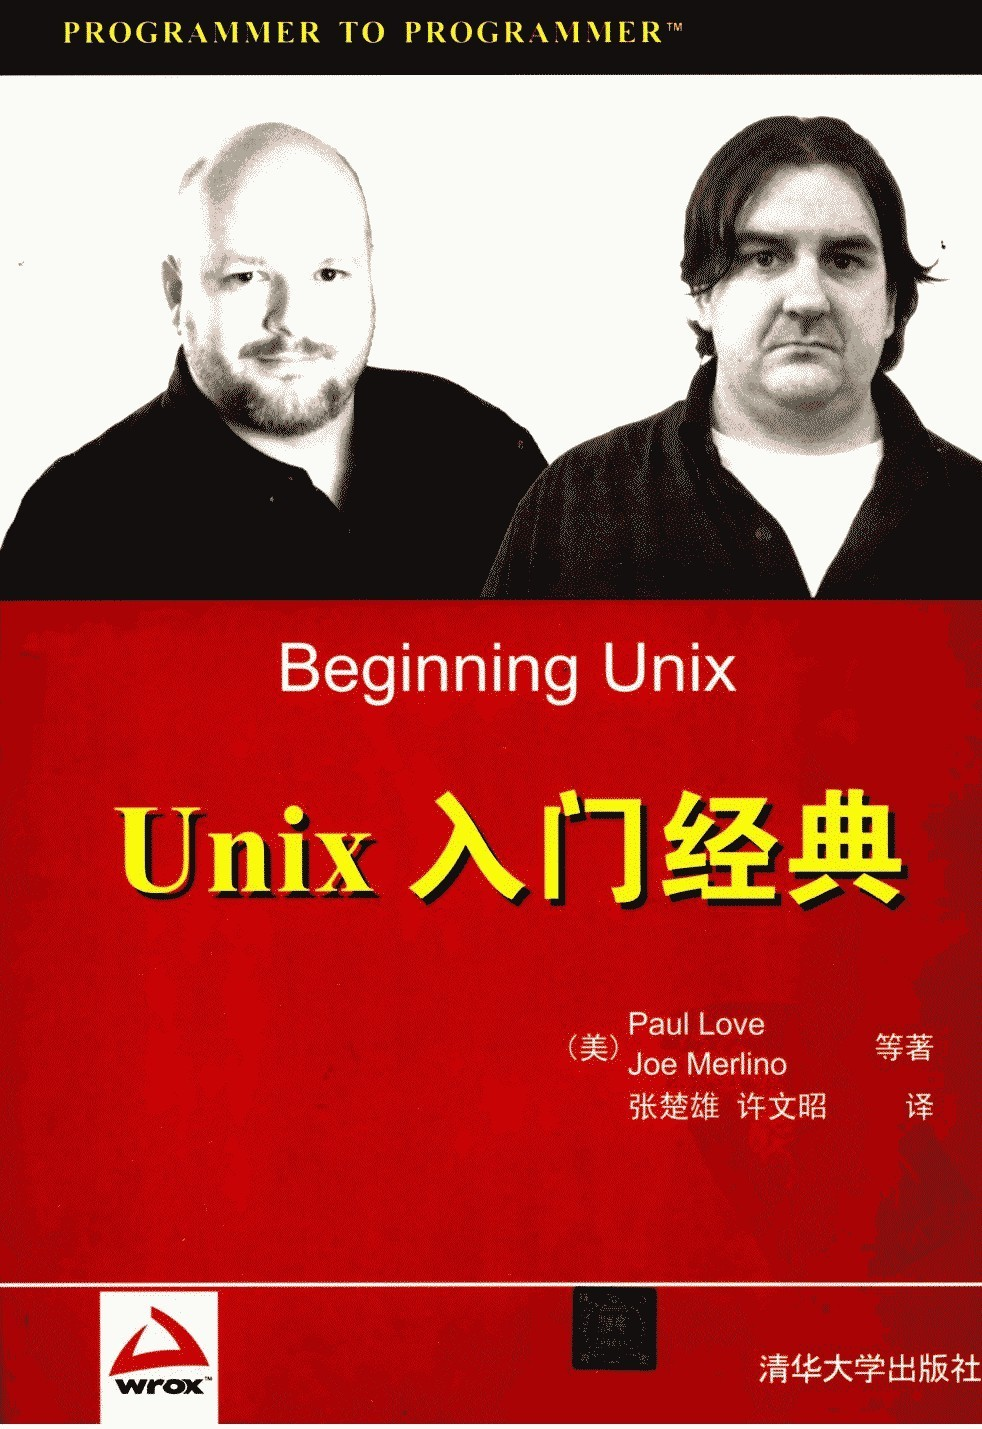
\includegraphics[width=0.4\textwidth]{c3.programming.linux.jpg}
  \end{figure}
\end{frame}

\section{学习方法}
\begin{frame}
  \frametitle{编程艺术 | 学习方法}
  \begin{block}{提问}
 学习编程的最佳方法是什么? 
  \end{block}
  \pause
  \begin{block}{回答}
    \begin{itemize}
      \item 取决于你要完成的任务
      \item 取决于你打算如何学习编程
      \item 取决于……
    \end{itemize}
  \end{block}
\end{frame}

\begin{frame}
  \frametitle{编程艺术 | 学习方法}
  \begin{block}{常见方法}
    \begin{itemize}
      \item 参加(XXX新手)培训班
      \item 阅读(XXX入门、30天学会XXX)书籍
      \item 死啃手册
      \item 拜师学艺
      \item 研究经典程序
      \item ……
      \item 组合多种方法
    \end{itemize}
  \end{block}
  \pause
  \begin{block}{\alert{五字真言}}
    \begin{itemize}
      \item 实践出真知!
      \item Experience is the best teacher.
      \item 不要只读书/看手册/读源代码,一定要亲自动手去编写、调试程序。
    \end{itemize}
  \end{block}
\end{frame}

\section{编写程序}
\begin{frame}
  \frametitle{编程艺术 | 编写程序 | \alert{基本流程(编辑-运行-修正)}}
  \begin{figure}
    \centering
    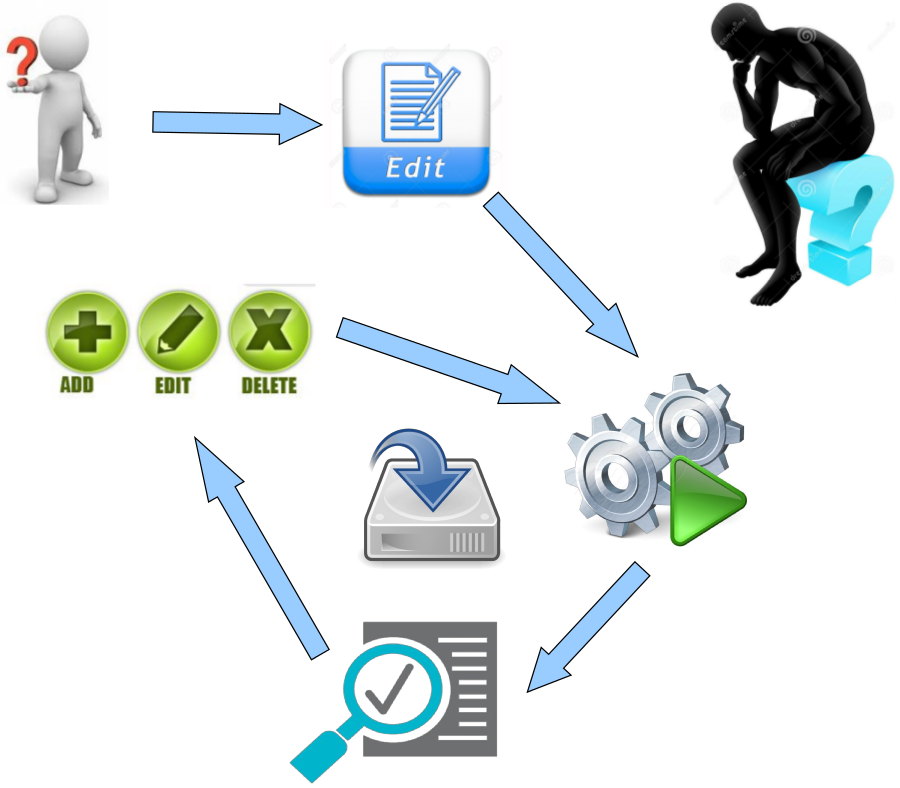
\includegraphics[width=0.72\textwidth]{c3.programming.cycle.png}
  \end{figure}
\end{frame}

\begin{frame}
  \frametitle{编程艺术 | 编写程序 | 版本控制}
  \begin{figure}
    \centering
    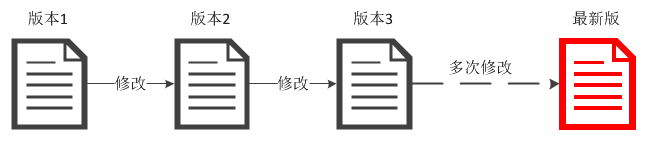
\includegraphics[width=0.7\textwidth]{c3.programming.version.01.png}\\
    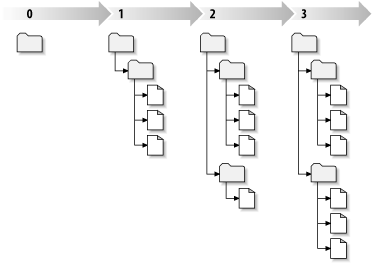
\includegraphics[width=0.8\textwidth]{c3.programming.version.02.png}\\
  \end{figure}
\end{frame}

\begin{frame}
  \frametitle{编程艺术 | 编写程序 | 版本控制}
  什么是版本控制?我真的需要吗?版本控制是一种记录若干文件内容变化,以便将来查阅特定版本修订情况的系统。\\
  \vspace{1em}
  如果你是位图形或网页设计师,可能会需要保存某一幅图片或页面布局文件的所有修订版本(这或许是你非常渴望拥有的功能)。采用版本控制系统(VCS,Version Control System)是个明智的选择。有了它你就可以将某个文件回溯到之前的状态,甚至将整个项目都回退到过去某个时间点的状态。你可以比较文件的变化细节,查出最后是谁修改了哪个地方,从而导致出现怪异问题,又是谁在何时报告了某个功能缺陷等等。使用版本控制系统通常还意味着,就算你乱来一气把整个项目中的文件改的改删的删,你也照样可以轻松恢复到原先的样子。但额外增加的工作量却微乎其微。\\
  \vspace{1em}
  许多人习惯用复制整个项目目录的方式来保存不同的版本,或许还会改名加上备份时间以示区别。这么做唯一的好处就是简单。不过坏处也不少:有时候会混淆所在的工作目录,一旦弄错文件丢了数据就没法撤销恢复。
\end{frame}

\begin{frame}
  \frametitle{编程艺术 | 编写程序 | 版本控制 | Git}
  Git是一个分散式版本控制软件,最初由林纳斯·托瓦兹(Linus Torvalds)创作,于2005年以GPL释出。最初目的是为更好地管理Linux内核开发而设计。\\
  \vspace{1em}
 Git是用于Linux内核开发的版本控制工具。与CVS、Subversion一类的集中式版本控制工具不同,它采用了分布式版本库的做法,不需要服务器端软件,就可以运作版本控制,使得源代码的发布和交流极其方便。Git的速度很快,这对于诸如Linux内核这样的大项目来说自然很重要。Git最为出色的是它的合并追踪(merge tracing)能力。\\
  \vspace{1em}
  在Git中的绝大多数操作都只需要访问本地文件和资源,不用连网。因为Git在本地磁盘上就保存着所有当前项目的历史更新,所以处理起来速度飞快。
\end{frame}

\begin{frame}
  \frametitle{编程艺术 | 编写程序 | 版本控制 | Git | 原理}
  Git和其他版本控制系统的主要差别在于,Git只关心文件数据的整体是否发生变化,而大多数其他系统则只关心文件内容的具体差异。\\
  \vspace{1em}
  这类系统(CVS,Subversion,Perforce,Bazaar等等)每次记录有哪些文件作了更新,以及都更新了哪些行的什么内容。\\
  \vspace{1em}
  Git并不保存这些前后变化的差异数据。实际上,Git更像是把变化的文件作快照后,记录在一个微型的文件系统中。每次提交更新时,它会纵览一遍所有文件的指纹信息并对文件作一快照,然后保存一个指向这次快照的索引。为提高性能,若文件没有变化,Git不会再次保存,而只对上次保存的快照作一链接。
\end{frame}

\begin{frame}[fragile]
  \frametitle{编程艺术 | 编写程序 | 版本控制 | Git | 范例}
\begin{lstlisting}[language=sh]
# 安装Git
sudo apt-get install git-core

# 使用帮助
man git
git --help
git help CMD

# 创建项目目录
mkdir ~/project
cd ~/project
\end{lstlisting}
\end{frame}

\begin{frame}[fragile]
  \frametitle{编程艺术 | 编写程序 | 版本控制 | Git | \alert{范例}}
\begin{lstlisting}[language=sh]
# 创建Git仓库(启动版本控制)
git init

# 创建编辑文件
vim script.pl
#print "Hello, world!";

# 添加需要进行版本控制的文件
git add script.pl
#git add .

# 提交改动信息
git commit -m "Say hello to the world."
\end{lstlisting}
\end{frame}

\begin{frame}[fragile]
  \frametitle{编程艺术 | 编写程序 | 版本控制 | Git | 范例}
\begin{lstlisting}[language=sh]
# 修改文件
vim script.pl
#把Hello替换成Bye

# 添加改动信息
git add .

# 提交改动信息
git commit -m "Bye to the world."

# 查看提交历史
git log

# 版本回退
git reset --hard ID #不需要全部ID,只需要有区分度的前几位即可
\end{lstlisting}
\end{frame}

\begin{frame}[fragile]
  \frametitle{编程艺术 | 编写程序 | 版本控制 | Git | 范例}
\begin{lstlisting}[language=sh]
# 创建test分支并切换过去
git checkout -b test
#相当于两步:git branch test; git checkout test

# 修改文件
vim script.pl
#添加一行:print "Bye, world!";

# 添加改动信息
git add .

# 提交改动信息
git commit -m "And bye to the world."
\end{lstlisting}
\end{frame}

\begin{frame}[fragile]
  \frametitle{编程艺术 | 编写程序 | 版本控制 | Git | 范例}
\begin{lstlisting}[language=sh]
# 切换回主分支
git checkout master

# 把test分支合并到主分支
git merge test
#可能需要手动修改后执行git add和git commit命令

# 删除test分支
git branch -d test
\end{lstlisting}
\end{frame}

\begin{frame}[fragile]
  \frametitle{编程艺术 | 编写程序 | 版本控制 | Git | 范例}
\begin{lstlisting}[language=sh]
# 查看状态
git status

# 查看提交日志
git log

# 查看修改内容
git diff

# 删除文件
git rm

# 查看/创建标签
git tag
\end{lstlisting}
\end{frame}

\begin{frame}[fragile]
  \frametitle{编程艺术 | 编写程序 | 版本控制 | Git | 范例}
\begin{lstlisting}[language=sh]
# 配置Git

#查看配置信息
git config --list

#彩色的 git 输出:
git config color.ui true
#显示历史记录时,只显示一行注释信息
git config format.pretty oneline

#配置个人信息等
git config --global user.name "Yixf"
git config --global user.email "yixf@example.com"
git config --global core.editor vim
\end{lstlisting}
\end{frame}

\begin{frame}[fragile]
  \frametitle{编程艺术 | 编写程序 | 版本控制 | Git | 范例}
\begin{lstlisting}[language=sh]
# 内置的图形化Git
gitk

# 忽略文件/文件夹
#.gitignore
videos/
*.pdf
*.doc
\end{lstlisting}
\end{frame}

\begin{frame}[fragile]
  \frametitle{编程艺术 | 编写程序 | 版本控制 | Git | 范例}
\begin{lstlisting}[language=sh]
# 克隆仓库
#克隆本地仓库
git clone /path/to/repository
#克隆远程服务器上的仓库到本地
git clone username@host:/path/to/repository

# 把本地已有的仓库和服务器上的仓库关联起来
git remote add origin <server>

# 把本地库的内容推送到远程库
git push origin master

# 把远程库的内容更新到本地库
git pull
\end{lstlisting}
\end{frame}

\begin{frame}
  \frametitle{编程艺术 | 编写程序 | 版本控制 | Git | \alert{范例}}
  \begin{figure}
    \centering
    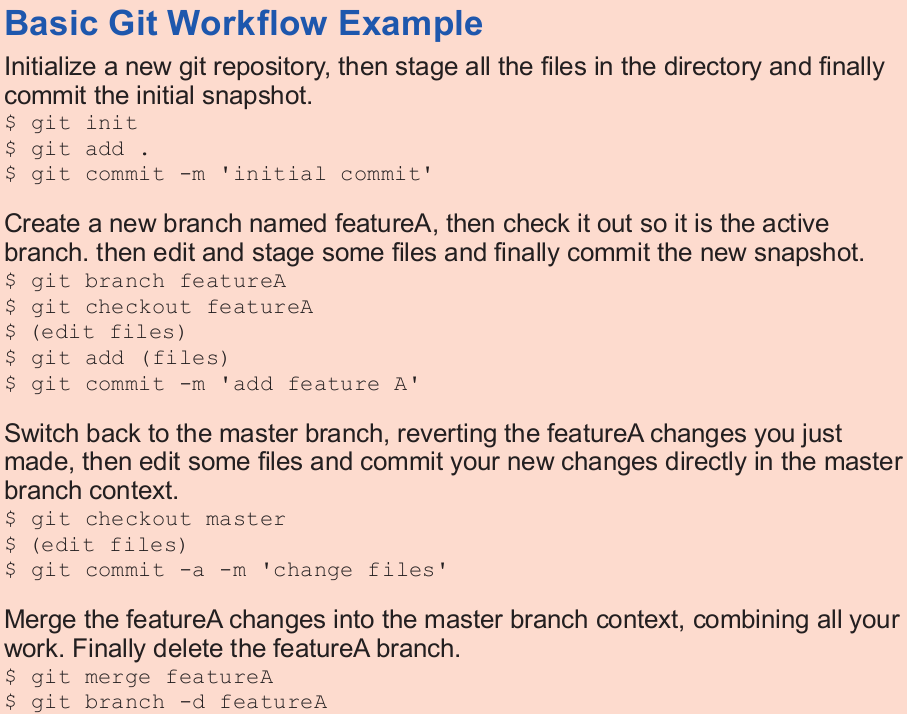
\includegraphics[width=0.8\textwidth]{c3.programming.git.png}
  \end{figure}
\end{frame}

\begin{frame}
  \frametitle{编程艺术 | 编写程序 | 版本控制 | GitHub}
  GitHub是一个共享虚拟主机服务,用于存放使用Git版本控制的软件代码和内容项目。\\
  \vspace{1em}
  GitHub同时提供付费账户和免费账户。这两种账户都可以建立公开的代码仓库,但是付费账户也可以建立私有的代码仓库。除了允许个人和组织建立和存取代码库以外,它也提供了一些方便社会化软件开发的功能,包括允许用户跟踪其他用户、组织、软件库的动态,对软件代码的改动和Bug提出评论等。GitHub也提供了图表功能,用于显示开发者们怎样在代码库上工作以及软件的开发活跃程度。\\
  \vspace{1em}
  截止到2015年,GitHub已经有超过九百万注册用户和2110万代码仓库。事实上已经成为了世界上最大的代码存放网站。\\
  \vspace{1em}
  GitHub里面的项目可以通过标准的Git命令进行访问和操作。同时,所有的Git命令都可以用到 GitHub项目上面。
\end{frame}

\begin{frame}
  \frametitle{编程艺术 | 编写程序 | 版本控制 | GitHub}
  \begin{figure}
    \centering
    \includegraphics[width=0.9\textwidth]{c3.programming.github.png}
  \end{figure}
\end{frame}

\begin{frame}
  \frametitle{编程艺术 | 编写程序 | 错误信息}
  \begin{itemize}
    \item 出错并不可怕!(【编程初期】出错是非常正常的。)
    \item 一定不要对错误信息视而不见!
    \item 从第一个错误开始,逐个进行修复。
    \item 必要时进行一定的猜测。
  \end{itemize}
\end{frame}

\begin{frame}[fragile]
  \frametitle{编程艺术 | 编写程序 | \alert{调试程序}}
  \begin{itemize}
    \item 使用Perl调试器:\verb|perl -d script.pl|。
    \item 在程序中加入print语句,输出中间值。
    \item 选择性地注释掉部分代码。
    \item 使用相关的模块:Benchmark,Data::Dumper,Smart::Comments,……
    \item 组合使用多种调试方法
    \item ……
  \end{itemize}
\end{frame}

\section{编程策略}
\begin{frame}
  \frametitle{编程艺术 | \alert{编程策略}}
  \begin{enumerate}
    \item 寻找现成的(免费/收费)程序:避免“重复发明轮子”
    \item 自己编写程序
      \begin{enumerate}
	\item 修改现成的程序(平时注意收集、整理程序)
	\item 充分利用已有模块,快速“拼凑”程序
	\item 从头编写完整的程序
      \end{enumerate}
    \item 请其他专家(无偿/有偿)编写程序
  \end{enumerate}
  \pause
  \begin{block}{注意}
    有时修改现成的程序可能会比从头编写一个完整的程序还要困难!
  \end{block}
\end{frame}

\section{编程过程}
\begin{frame}
  \frametitle{编程艺术| 编程过程 | 实例}
  \begin{center}
    {\Large 计算一个DNA序列中调控元件的数目。}
  \end{center}
  \begin{figure}
    \centering
    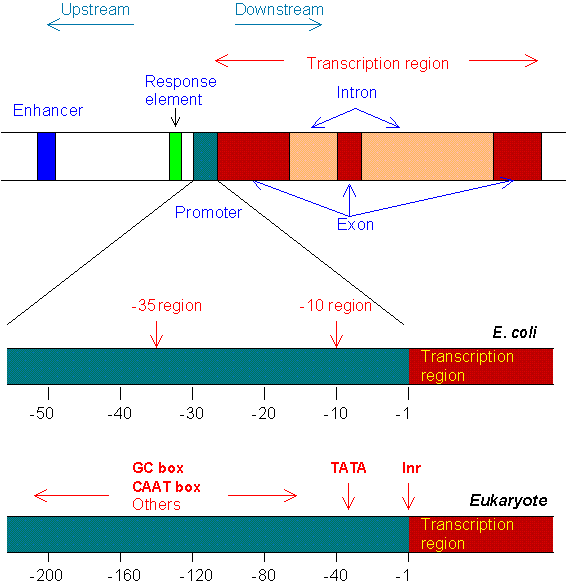
\includegraphics[width=0.55\textwidth]{c3.programming.re.01.png}
  \end{figure}
\end{frame}

\begin{frame}
  \frametitle{编程艺术 | 编程过程 | \alert{基本步骤}}
  \begin{itemize}
    \item 分析任务属性,对其进行充分的理解(数量、频率、时间等)
    \item 确定输入数据,对其进行充分理解(数据量、格式等)
    \item 对程序进行整理构思(算法、数据结构等)
    \item 确定输出数据,包括输出方法(文件、图形化展示、管道)、格式等
    \item 进一步改善整体构思,根据输入、输出等信息添加细节内容
    \item 必要时编写伪代码整理思路
    \item 最后才是动手编写程序代码
  \end{itemize}
\end{frame}

\begin{frame}
  \frametitle{编程艺术 | 编程过程 | \alert{构思}}
  \begin{itemize}
    \item 程序构思:在实际编程前首先要完成的关键步骤
    \item 分析任务属性:任务数量、任务频率、解决任务的时间限制等
    \item 确定输入数据:数据来源(文件、输入等)、数据数量、数据校验(文件存不存在、格式对不对)等
    \item 选择正确/合适的算法(速度、优劣):针对每一个调控元件,在DNA序列中从头到尾进行查找;针对DNA序列的每一个位置,对每个调控元件进行查找
    \item 确定输出数据:输出形式、数据格式、人性化输出(用户提供文件名、易于解读……)等
    \item 选择编程范式,命令式编程(把一个大的问题/程序分割成多个微小、但却相互关联配合的部分/子程序):程序式编程,面向对象编程
    \item 编写伪代码:整理思路、优化构思、调整细节……
  \end{itemize}
\end{frame}

\begin{frame}
  \frametitle{编程艺术 | 编程过程 | 算法}
  在数学和计算机科学/算学之中,算法(algorithm)为一个计算的具体步骤,常用于计算、数据处理和自动推理。精确而言,算法是一个表示为有限长列表的有效方法。算法应包含清晰定义的指令用于计算函数。\\
  \vspace{1em}
  算法中的指令描述的是一个计算,当其运行时能从一个初始状态和初始输入(可能为空)开始,经过一系列有限而清晰定义的状态最终产生输出并停止于一个终态。\\
  \vspace{1em}
  程序所做的事情:获取文件、打开文件、读入数据、进行计算、输出结果;而算法就是此过程中计算的思路。
\end{frame}

\begin{frame}
  \frametitle{编程艺术 | 编程过程 | 伪代码}
  伪代码(pseudocode),又称为虚拟代码,是高层次描述算法的一种方法。它不是一种现实存在的编程语言;它可能综合使用多种编程语言的语法、保留字,甚至会用到自然语言。\\
  \vspace{1em}
  它以编程语言的书写形式指明算法的职能。相比于程序语言,它更类似自然语言。它是半形式化、不标准的语言。我们可以将整个算法运行过程的结构用接近自然语言的形式(这里可以使用任何一种作者熟悉的文字,例如中文、英文,重点是将程序的意思表达出来)描述出来。使用伪代码,可以帮助我们更好得表述算法,不用拘泥于具体的实现。\\
  \vspace{1em}
  人们在用不同的编程语言实现同一个算法时意识到,他们做出来的实现(而非功能)很不同。程序员要理解一个用他并不熟悉的编程语言编写的程序,可能是很困难的,因为程序语言的形式限制了程序员对程序关键部分的理解。伪代码就这样应运而生了。\\
  \vspace{1em}
  当考虑算法功能(而不是其语言实现)时,伪代码常常得到应用。计算机科学在教学中通常使用伪代码,以使得所有的程序员都能理解。
\end{frame}

\begin{frame}[fragile]
  \frametitle{编程艺术 | 编程过程 | 伪代码}
伪代码是介于自然语言和编程语言之间的一种“中间语言”。
  \begin{block}{代码}
\begin{lstlisting}[language=Perl]
sub getanswer {
  print "Type in your answer here :";  
  my $answer = <STDIN>;
  chomp $answer;
  return $answer;
}
\end{lstlisting}
\end{block}
\pause
\begin{block}{伪代码}
\begin{lstlisting}[language=]
getanswer
\end{lstlisting}
\end{block}
\end{frame}

\begin{frame}[fragile]
  \frametitle{编程艺术 | 编程过程 | \alert{伪代码}}
\begin{lstlisting}[language=Perl]
get the name of DNAfile from the user

read in the DNA from the DNAfile

for each regulatory element
  if element is in DNA, then
    add one to the count

print count
\end{lstlisting}
\end{frame}

\begin{frame}[fragile]
  \frametitle{编程艺术 | 编程过程 | \alert{注释}}
  \begin{itemize}
    \item 注释是源代码的一部分,旨在帮助用户/程序员理解程序
    \item 从\verb|#|开始到行末的所有内容都被看做是注释,会被Perl解释器忽略掉
    \item 首行的\verb|#!/usr/bin/perl|不是注释,不会被Perl解释器忽略掉
    \item 注释内容:程序的目的、整体构思、使用实例、细节注释等
    \item 牢记:代码不止是被计算机看的,也会被人查看
    \item 可以通过注释掉伪代码把它们保留在程序中
  \end{itemize}
\end{frame}

\section{回顾与总结}
\subsection{总结}
\begin{frame}
  \frametitle{编程艺术 | 总结}
  \begin{block}{知识点}
    \begin{itemize}
      \item 学习编程的方法:培训班、读书、看手册、拜师、研究程序、……
      \item 编程的基本流程:编辑-运行-修正
      \item 版本控制:Git,GitHub
      \item 调试程序:调试器、print、注释、模块、……
      \item 编程策略:找现成的程序、自己编写程序、请别人帮忙、……
      \item 编程的基本步骤:构思(输入、算法、输出)、编程
      \item 编程前:伪代码;编程中:注释
    \end{itemize}
  \end{block}
  \pause
  \begin{block}{技能}
    \begin{itemize}
      %\item 能够自学一门编程语言
      \item 熟练应用编程的基本策略、步骤和流程
      \item 能够使用Git和GitHub进行版本控制
      \item 能够用不同的方法调试程序
      %\item 能够针对不同的问题采用不同的编程策略
      %\item 能够熟练撰写伪代码
    \end{itemize}
  \end{block}
\end{frame}

\subsection{思考题}
\begin{frame}
  \frametitle{编程艺术 | 思考题}
  \begin{enumerate}
    \item 总结学习编程语言的方法。
    \item 编写程序的基本流程是什么?
    \item 如何使用Git进行版本控制?
    \item 总结调试程序的方法。
    \item 总结常用的编程策略。
    \item 编程的基本步骤是什么?需要构思哪些内容?
    \item 使用伪代码和注释有哪些优势?
  \end{enumerate}
\end{frame}

\begin{frame}
  \frametitle{下节预告}
  \begin{block}{编程相关}
    回顾shell/Perl中的以下知识点:
    \begin{itemize}
      \item 变量
      \item 数组
    \end{itemize}
  \end{block}
  \begin{block}{生物学相关}
    回顾生物学中的以下知识点:
    \begin{itemize}
      \item DNA的组成
      \item DNA的转录
      \item DNA的反向互补
      \item 蛋白质的组成
    \end{itemize}
  \end{block}
\end{frame}



\section*{Acknowledgements}
\begin{frame}
  \frametitle{Powered by}
  \begin{center}
    
\includegraphics[width=9cm]{power.png}
  \end{center}
\end{frame}

\end{document}

